\documentclass[10pt]{article}
\usepackage{tikz}
\usetikzlibrary{shapes.misc}
\usepackage[margin=0cm]{geometry}
\pagestyle{empty}
\tikzstyle{every node}=[cross out, draw, red]

\begin{document}

\vspace*{\fill}
\begin{center}
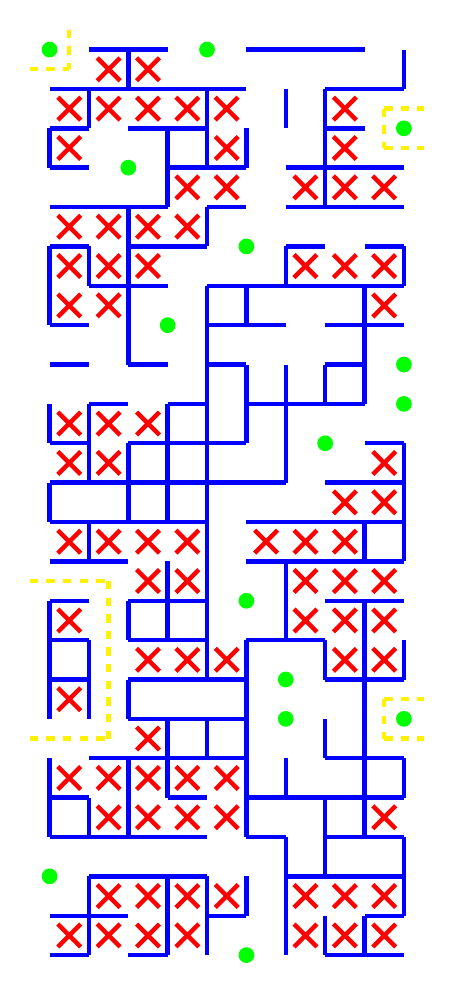
\begin{tikzpicture}[x=0.5cm, y=-0.5cm, ultra thick, blue]
% Walls
    \draw (1,0) -- (3,0);
    \draw (5,0) -- (8,0);
    \draw (0,1) -- (5,1);
    \draw (7,1) -- (9,1);
    \draw (0,2) -- (1,2);
    \draw (2,2) -- (4,2);
    \draw (7,2) -- (8,2);
    \draw (0,3) -- (1,3);
    \draw (3,3) -- (5,3);
    \draw (6,3) -- (9,3);
    \draw (0,4) -- (3,4);
    \draw (4,4) -- (5,4);
    \draw (6,4) -- (9,4);
    \draw (0,5) -- (1,5);
    \draw (2,5) -- (4,5);
    \draw (6,5) -- (7,5);
    \draw (8,5) -- (9,5);
    \draw (1,6) -- (3,6);
    \draw (4,6) -- (9,6);
    \draw (0,7) -- (1,7);
    \draw (4,7) -- (6,7);
    \draw (7,7) -- (9,7);
    \draw (0,8) -- (1,8);
    \draw (2,8) -- (3,8);
    \draw (4,8) -- (5,8);
    \draw (7,8) -- (8,8);
    \draw (1,9) -- (2,9);
    \draw (3,9) -- (4,9);
    \draw (5,9) -- (8,9);
    \draw (0,10) -- (1,10);
    \draw (2,10) -- (5,10);
    \draw (8,10) -- (9,10);
    \draw (0,11) -- (6,11);
    \draw (7,11) -- (9,11);
    \draw (0,12) -- (4,12);
    \draw (5,12) -- (9,12);
    \draw (0,13) -- (2,13);
    \draw (5,13) -- (9,13);
    \draw (0,14) -- (1,14);
    \draw (2,14) -- (4,14);
    \draw (7,14) -- (9,14);
    \draw (0,15) -- (1,15);
    \draw (2,15) -- (4,15);
    \draw (5,15) -- (7,15);
    \draw (0,16) -- (1,16);
    \draw (2,16) -- (5,16);
    \draw (7,16) -- (9,16);
    \draw (2,17) -- (5,17);
    \draw (1,18) -- (5,18);
    \draw (7,18) -- (9,18);
    \draw (0,19) -- (1,19);
    \draw (3,19) -- (4,19);
    \draw (5,19) -- (9,19);
    \draw (0,20) -- (4,20);
    \draw (5,20) -- (6,20);
    \draw (7,20) -- (9,20);
    \draw (1,21) -- (4,21);
    \draw (6,21) -- (9,21);
    \draw (0,22) -- (2,22);
    \draw (4,22) -- (5,22);
    \draw (8,22) -- (9,22);
    \draw (0,23) -- (1,23);
    \draw (2,23) -- (3,23);
    \draw (7,23) -- (9,23);
    \draw (0,2) -- (0,3);
    \draw (0,5) -- (0,7);
    \draw (0,9) -- (0,10);
    \draw (0,11) -- (0,12);
    \draw (0,14) -- (0,17);
    \draw (0,18) -- (0,20);
    \draw (1,1) -- (1,2);
    \draw (1,5) -- (1,6);
    \draw (1,9) -- (1,11);
    \draw (1,12) -- (1,13);
    \draw (1,15) -- (1,17);
    \draw (1,19) -- (1,20);
    \draw (1,21) -- (1,23);
    \draw (2,0) -- (2,1);
    \draw (2,4) -- (2,8);
    \draw (2,10) -- (2,12);
    \draw (2,14) -- (2,15);
    \draw (2,16) -- (2,17);
    \draw (2,18) -- (2,20);
    \draw (3,2) -- (3,4);
    \draw (3,9) -- (3,12);
    \draw (3,13) -- (3,15);
    \draw (3,17) -- (3,19);
    \draw (3,21) -- (3,23);
    \draw (4,1) -- (4,3);
    \draw (4,4) -- (4,5);
    \draw (4,6) -- (4,16);
    \draw (4,17) -- (4,18);
    \draw (4,21) -- (4,23);
    \draw (5,2) -- (5,3);
    \draw (5,6) -- (5,7);
    \draw (5,8) -- (5,10);
    \draw (5,15) -- (5,20);
    \draw (5,21) -- (5,22);
    \draw (6,1) -- (6,2);
    \draw (6,5) -- (6,6);
    \draw (6,8) -- (6,11);
    \draw (6,13) -- (6,15);
    \draw (6,18) -- (6,19);
    \draw (6,20) -- (6,23);
    \draw (7,1) -- (7,4);
    \draw (7,8) -- (7,9);
    \draw (7,15) -- (7,16);
    \draw (7,17) -- (7,18);
    \draw (7,19) -- (7,21);
    \draw (7,22) -- (7,23);
    \draw (8,6) -- (8,9);
    \draw (8,12) -- (8,13);
    \draw (8,14) -- (8,20);
    \draw (8,22) -- (8,23);
    \draw (9,0) -- (9,1);
    \draw (9,5) -- (9,6);
    \draw (9,10) -- (9,13);
    \draw (9,15) -- (9,16);
    \draw (9,18) -- (9,19);
    \draw (9,20) -- (9,22);
% Pillars
    \fill[green] (0,0) circle(0.2);
    \fill[green] (4,0) circle(0.2);
    \fill[green] (9,2) circle(0.2);
    \fill[green] (2,3) circle(0.2);
    \fill[green] (5,5) circle(0.2);
    \fill[green] (3,7) circle(0.2);
    \fill[green] (9,8) circle(0.2);
    \fill[green] (9,9) circle(0.2);
    \fill[green] (7,10) circle(0.2);
    \fill[green] (5,14) circle(0.2);
    \fill[green] (6,16) circle(0.2);
    \fill[green] (6,17) circle(0.2);
    \fill[green] (9,17) circle(0.2);
    \fill[green] (0,21) circle(0.2);
    \fill[green] (5,23) circle(0.2);
% Inner points in accessible cul-de-sacs
    \node at (1.5,0.5) {};
    \node at (2.5,0.5) {};
    \node at (0.5,1.5) {};
    \node at (1.5,1.5) {};
    \node at (2.5,1.5) {};
    \node at (3.5,1.5) {};
    \node at (4.5,1.5) {};
    \node at (7.5,1.5) {};
    \node at (0.5,2.5) {};
    \node at (4.5,2.5) {};
    \node at (7.5,2.5) {};
    \node at (3.5,3.5) {};
    \node at (4.5,3.5) {};
    \node at (6.5,3.5) {};
    \node at (7.5,3.5) {};
    \node at (8.5,3.5) {};
    \node at (0.5,4.5) {};
    \node at (1.5,4.5) {};
    \node at (2.5,4.5) {};
    \node at (3.5,4.5) {};
    \node at (0.5,5.5) {};
    \node at (1.5,5.5) {};
    \node at (2.5,5.5) {};
    \node at (6.5,5.5) {};
    \node at (7.5,5.5) {};
    \node at (8.5,5.5) {};
    \node at (0.5,6.5) {};
    \node at (1.5,6.5) {};
    \node at (8.5,6.5) {};
    \node at (0.5,9.5) {};
    \node at (1.5,9.5) {};
    \node at (2.5,9.5) {};
    \node at (0.5,10.5) {};
    \node at (1.5,10.5) {};
    \node at (8.5,10.5) {};
    \node at (7.5,11.5) {};
    \node at (8.5,11.5) {};
    \node at (0.5,12.5) {};
    \node at (1.5,12.5) {};
    \node at (2.5,12.5) {};
    \node at (3.5,12.5) {};
    \node at (5.5,12.5) {};
    \node at (6.5,12.5) {};
    \node at (7.5,12.5) {};
    \node at (2.5,13.5) {};
    \node at (3.5,13.5) {};
    \node at (6.5,13.5) {};
    \node at (7.5,13.5) {};
    \node at (8.5,13.5) {};
    \node at (0.5,14.5) {};
    \node at (6.5,14.5) {};
    \node at (7.5,14.5) {};
    \node at (8.5,14.5) {};
    \node at (2.5,15.5) {};
    \node at (3.5,15.5) {};
    \node at (4.5,15.5) {};
    \node at (7.5,15.5) {};
    \node at (8.5,15.5) {};
    \node at (0.5,16.5) {};
    \node at (2.5,17.5) {};
    \node at (0.5,18.5) {};
    \node at (1.5,18.5) {};
    \node at (2.5,18.5) {};
    \node at (3.5,18.5) {};
    \node at (4.5,18.5) {};
    \node at (1.5,19.5) {};
    \node at (2.5,19.5) {};
    \node at (3.5,19.5) {};
    \node at (4.5,19.5) {};
    \node at (8.5,19.5) {};
    \node at (1.5,21.5) {};
    \node at (2.5,21.5) {};
    \node at (3.5,21.5) {};
    \node at (4.5,21.5) {};
    \node at (6.5,21.5) {};
    \node at (7.5,21.5) {};
    \node at (8.5,21.5) {};
    \node at (0.5,22.5) {};
    \node at (1.5,22.5) {};
    \node at (2.5,22.5) {};
    \node at (3.5,22.5) {};
    \node at (6.5,22.5) {};
    \node at (7.5,22.5) {};
    \node at (8.5,22.5) {};
% Entry-exit paths without intersections
    \draw[dashed, yellow] (-0.5,0.5) -- (0.5,0.5);
    \draw[dashed, yellow] (8.5,1.5) -- (9.5,1.5);
    \draw[dashed, yellow] (8.5,2.5) -- (9.5,2.5);
    \draw[dashed, yellow] (-0.5,13.5) -- (1.5,13.5);
    \draw[dashed, yellow] (8.5,16.5) -- (9.5,16.5);
    \draw[dashed, yellow] (-0.5,17.5) -- (1.5,17.5);
    \draw[dashed, yellow] (8.5,17.5) -- (9.5,17.5);
    \draw[dashed, yellow] (0.5,-0.5) -- (0.5,0.5);
    \draw[dashed, yellow] (1.5,13.5) -- (1.5,17.5);
    \draw[dashed, yellow] (8.5,1.5) -- (8.5,2.5);
    \draw[dashed, yellow] (8.5,16.5) -- (8.5,17.5);
\end{tikzpicture}
\end{center}
\vspace*{\fill}

\end{document}
